%----------createInterface----------------------------------------
\op
{createInterface}
{creates a new interface}
{createInterface(Package selectedEObject, String nameValue, String idValue)}
{The package providing the container for the newly created interface.}
{
\begin{itemize}
 \item nameValue/newName: The name of the newly created interface
 \item idValue/newID: The id of the newly created interface
\end{itemize}
}
{There is no interface whose name equals the parameter-value of 'newName' (see
\ref{subsec:checkOtherNames})}
{Only the name and the id will be set via input data. Visibility will be set
with a default value as defined with the diagram editor in the image below.}
\begin{figure}[H]
  \centering
  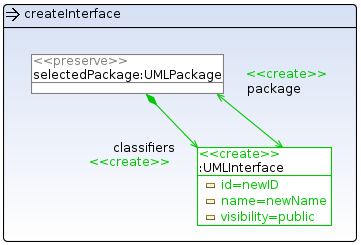
\includegraphics[width=0.65\textwidth]{pics/createInterface.png}
  \caption{createInterface}
  \label{createInterface}
\end{figure}
%----------deleteInterface----------------------------------------
\op
{deleteInterface}
{Deletes an interface}
{deleteInterface(Interface selectedEObject)}
{The interface which should be deleted} {-}
{-}
{For a better readability this is a simplified version of the
'deleteInterface'-transformation and will only cover cases where the
interfac has no containments and no references to other elements. Such a
complex transformation rule exits but won't be listed here.}
\begin{figure}[H]
  \centering
  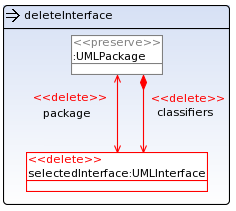
\includegraphics[width=0.4\textwidth]{pics/deleteInterface_emptyAndUnreferenced.png}
  \caption{deleteInterface}
  \label{deleteInterface}
\end{figure}

%----------editInterfaceName----------------------------------------
\op
{editInterfaceName}
{edits the name of an interface}
{editInterfaceName(Interface selectedEObject, String nameValue)}
{The interface whose name should be renamed.}
{
\begin{itemize}
 \item nameValue/newName: The new name
\end{itemize}
}
{There is no interface in the same package whose name equals the parameter-value of
'newName' (see
\ref{subsec:checkOtherNames})}
{The \textless\textless create\textgreater\textgreater  -symbol in the image
means that even if the attribute exists its value will be overwritten.
'newName' is the placeholder for the input name.}
\begin{figure}[H]
  \centering
  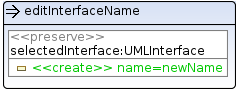
\includegraphics[width=0.4\textwidth]{pics/editInterfaceName.png}
  \caption{editInterfaceName}
  \label{editInterfaceName}
\end{figure}
%----------editInterfaceVisibility----------------------------------------
\op
{editInterfaceVisibility}
{edits the visibility of an interface}
{editInterfaceVisibility(Interface selectedEObject, Visibility visibilityValue)}
{The interface whose visibility should be edited.}
{
\begin{itemize}
 \item visibilityValue/visibility: The new visiblility
\end{itemize}
}
{-}
{The \textless\textless create\textgreater\textgreater  -symbol in the image
means that even if the attribute exists its value will be overwritten.
'visibility' is the placeholder for the input visibility value.}
\begin{figure}[H]
  \centering
  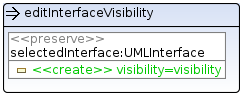
\includegraphics[width=0.4\textwidth]{pics/editInterfaceVisibility.png}
  \caption{editInterfaceVisibility}
  \label{editInterfaceVisibility}
\end{figure}
%----------moveInterface----------------------------------------
\op
{moveInterface}
{moves an interface from a package to another package}
{moveInterface(Interface selectedEObject, Package tgt)}
{The interface which should be moved.}
{
\begin{itemize}
 \item tgt/tgt[moveInterface]: the target package
\end{itemize}
}
{There is no interface with the same name in the target context (see
\ref{subsec:checkOtherNames})}
{Only references will change}
\begin{figure}[H]
  \centering
  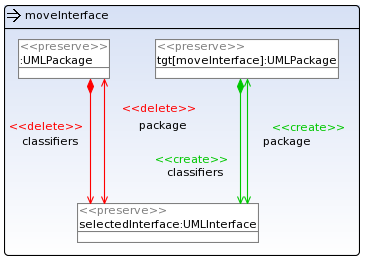
\includegraphics[width=0.65\textwidth]{pics/moveInterface.png}
  \caption{moveInterface}
  \label{moveInterface}
\end{figure}